\begin{figure}
    \centering
    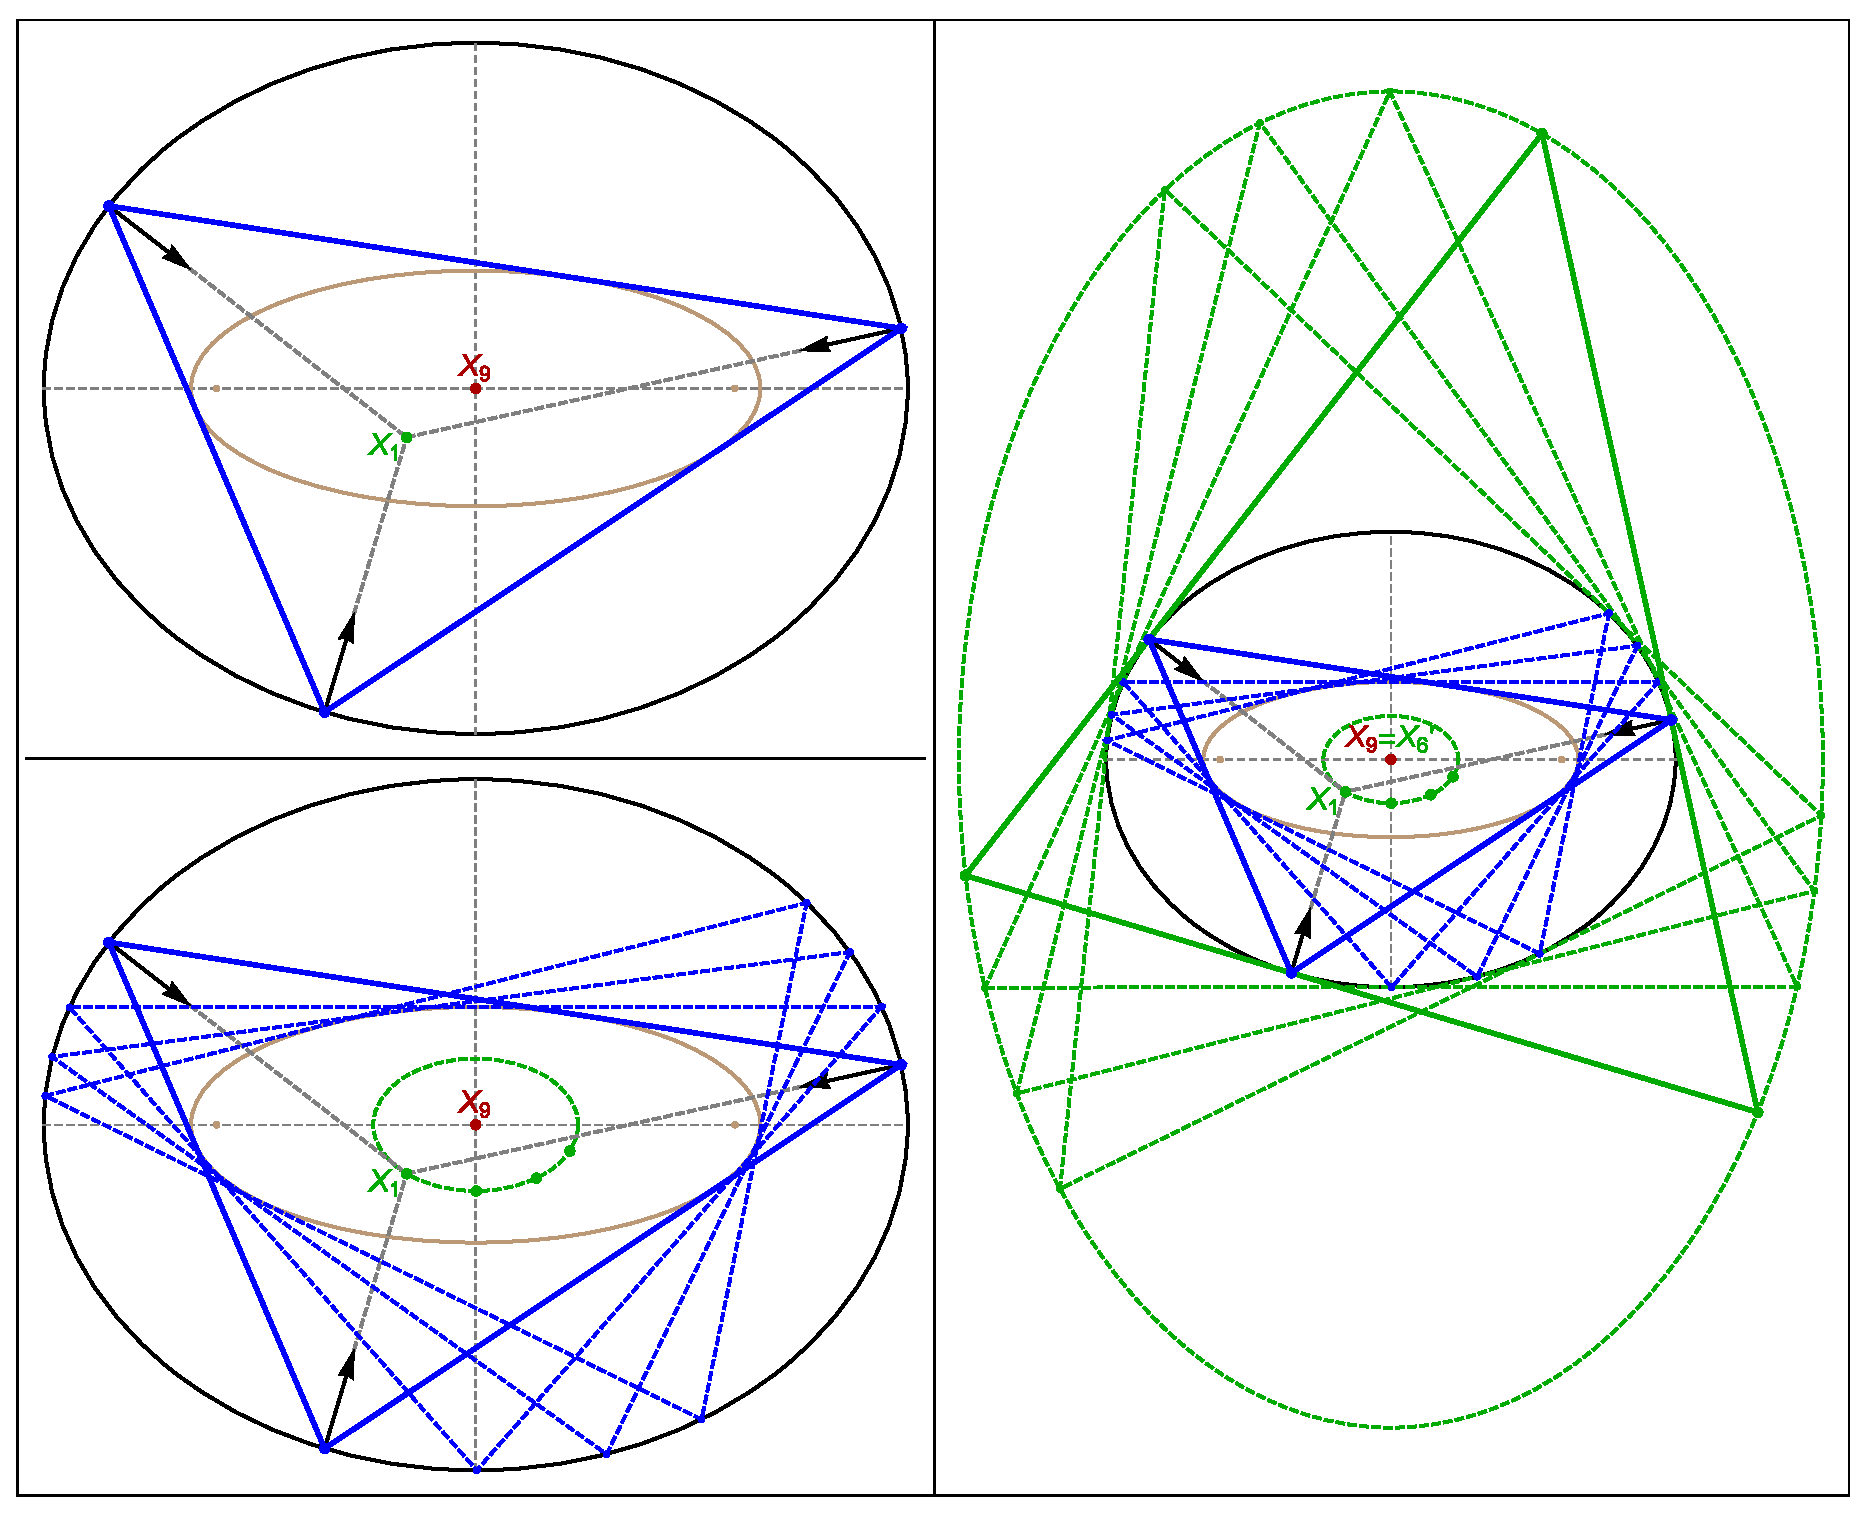
\includegraphics[width=\textwidth]{pics_03_080_billiard_grid.eps}
    \caption{\textbf{Top Left:} An elliptic billiard 3-periodic (solid blue) is shown inscribed in an outer ellipse (black) and a confocal caustic (brown). Graves' theorem implies its internal angles will be bisected by ellipse normals (black arrows). Also shown is the incenter $X_1$ defined as the intersection of said bisectors. \textbf{Bottom Left:} Poncelet's porism implies a 1d family of such triangles exists. Some samples are shown (dashed blue). A classic invariant is  perimeter. The Mittenpunkt $X_9$ remains stationary at the center. The incenter $X_1$ sweeps an ellipse (dashed green). \textbf{Right:} The excentral triangle (solid green) has sides perpendicular to the bisectors. Over billiard 3-periodics, the excentral is of variable perimeter. Its vertices (known as the ``excenters'') also sweep an ellipse (dashed green) whose aspect ratio is the reciprocal of that of the incenter locus. The Symmedian point $X_6'$ of the excentral triangle coincides with $X_9$ of the reference and is therefore stationary.}
    \label{fig:billiard-grid}
\end{figure}

Henceforth let {\em billiard 3-periodics} refer to the 1d family of Poncelet triangles interscribed between pair of confocal ellipses $\E$ and $\E_c$ given by:
\[ \E:\frac{x^2}{a^2}+\frac{y^2}{b^2}-1=0,\;\;\;\E_c:\frac{x^2}{a_c^2}+\frac{y^2}{b_c^2}-1=0\]
where $c^2=a^2-b^2=a_c^2-b_c^2$. Referring to \cref{fig:billiard-grid}:

\begin{theorem}
Over billiard 3-periodics, the locus of the incenter $X_1$ and excenter are ellipses $\E_1$ and $\E'$ concentric and axis-parallel with the confocal pair whose axes $(a_1,b_1)$ and $(a',b')$ are given by:
\begin{align*}
a_1 =& \frac{\delta-b^2 }{a},\;\;\;b_1=\frac{a^2-\delta}{b}\\ 
a'= &\frac{{b}^{2}+\delta}{a},\;\;\;b'=\frac{{a}^{2}+\delta}{b}
\end{align*}
where $\delta=\sqrt{a^4-a^2b^2+b^4}$ is called here the {\em Darboux} constant. 
Furthermore, $\E_1$ and $\E'$ have reciprocal aspect ratios, i.e., $a_1/b_1=b_e/a_e$.
\label{thm:03_incenter_excenter}
\end{theorem}

The Mittenpunkt $X_9$ is a triangle center where lines from each excenter thru the side midpoint meet. Referring to \cref{fig:x9}:

\begin{theorem}
Over the family of 3-periodics in the elliptic billiard, $X_9$ is stationary at the common center.
\end{theorem}

An elegant syntethic proof was kindly contributed by Olga Romaskevich in \cite{olga19_mitten}:

\begin{proof}
Let $\E$ be the outer ellipse in the confocal pair, $O$ their center, and $E_i$ the excenters, $i=1,2,3$. Let $M_i$ denote the midpoint of the chord between tangents to $\E$ seen from an $E_i$. Let $E_i' M_i'$ denote the image of lines $E_i M_i$ under an affine transform which sends $\E$ to a circle $\C'$ centered on $O'$. Since affine transformations preserve length ratios, lines $E_i' M_i'$ will also cut the chords between tangents to $\C'$ seend from the $E_i'$ in half. By circular symmetry, all said lines must meet in $O'$, which is fixed. Since the affine group also preserves line intersections, the result follows.
\end{proof}

\begin{figure}
     \centering
    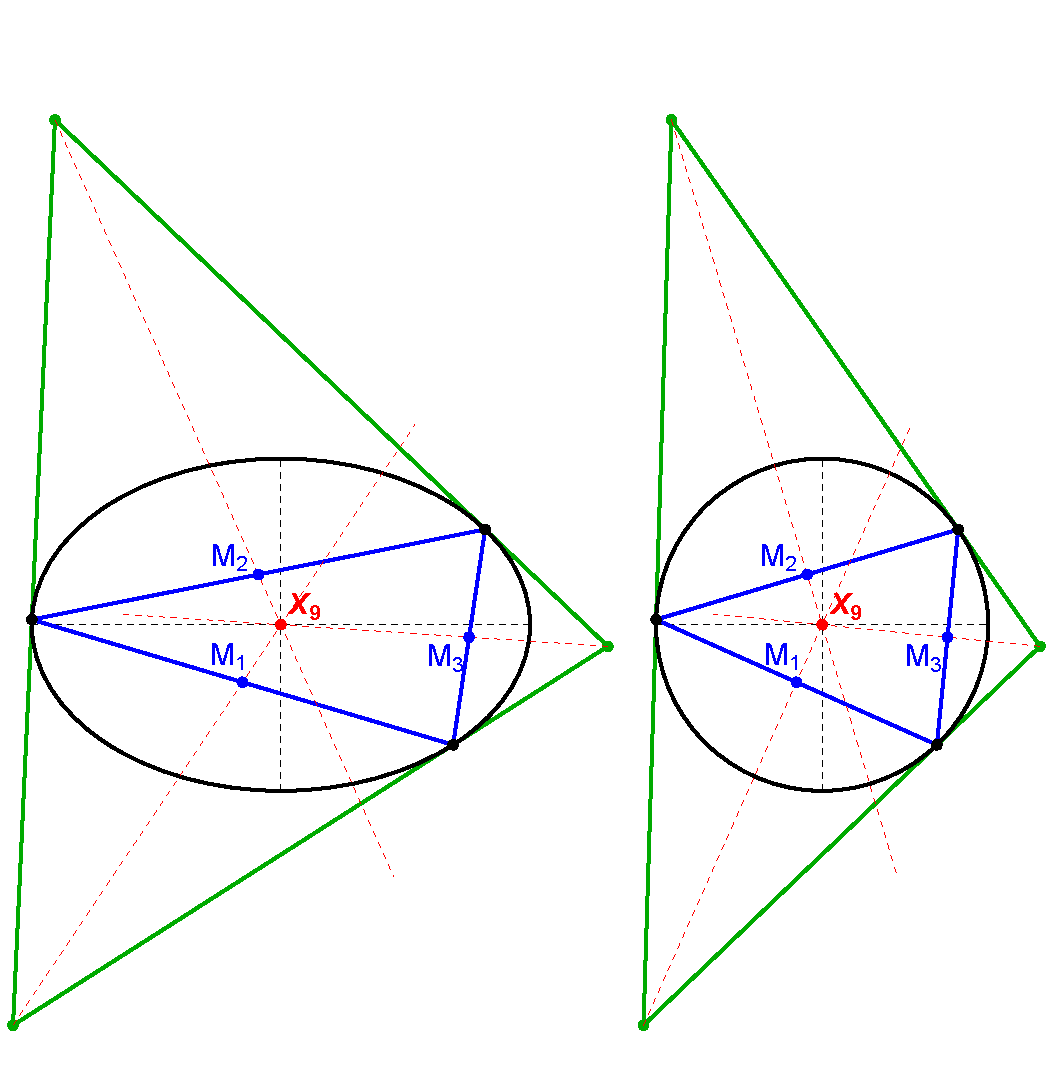
\includegraphics[width=\linewidth]{pics_03_090_mitten_proof.pdf}    
     \caption{\textbf{Left}: 3-periodic billiard triangle (blue), its excentral triangle (green), and the construction for $X_9$, the Mittenpunkt, which remains stationary at the center of the billiard (black). \textbf{Right}: affine image which sends the billiard to a circle. Lines connecting the image of excenters to the center must pass thru side midpoints and will therefore remain stationary.  % done
     \href{https://youtu.be/tMrBqfRBYik}{Video}}
     \label{fig:x9} 
\end{figure}

Referring to \cref{fig:radii}:

\begin{theorem}
\label{thm:rovR}
$r/R$ is invariant over the 3-periodic orbit family and given by
\begin{equation}
\label{eqn:rovR}
\frac{r}{R}=\frac{2 (\delta-b^2)(a^2-\delta)}{(a^2-b^2)^2}.
\end{equation}
\end{theorem}

\begin{proof}
Let $r$ and $R$ be the radius of the incircle and circumcircle, respectively. For any triangle \cite{coxeter67} we have

\begin{equation*}
 r R=\frac{s_1s_2s_3}{2 L}, 
\end{equation*}

\noindent where $L=s_1+s_2+s_3$ is the perimeter, constant for 3-periodic orbits; see equation \eqref{eqn:perimeter}. Therefore,

\begin{equation}
\frac{r}{R}=\frac{1}{2L} \frac{s_1s_2s_3}{R^2}\cdot
\label{eqn:rovR-cas}
\end{equation}

\textcolor{red}{ronaldo improve?}
Next, with $P_1=(a,0)$, obtain a {\em candidate} expression for $r/R$. This yields \eqref{eqn:rovR} exactly. Using explicit expressions for orbit vertices (see Appendix~\ref{app:orbit-vertices}), derive an expression for the square of the right-hand side of \eqref{eqn:rovR-cas} as a function of $x_1$ and subtract from it the square of \eqref{eqn:rovR}. It can be shown $\left(s_1s_2s_3/R^2\right)^2$ is rational on $x_1$ \cite{reznik2020-loci}. For simplification, use $R=s_1 s_2 s_3/(4A)$, where $A$ is the triangle area. With a computer algebra system (CAS), show said difference is identically zero for all $x_1\in(-a,a)$.
\end{proof}


\begin{figure}
    \centering
    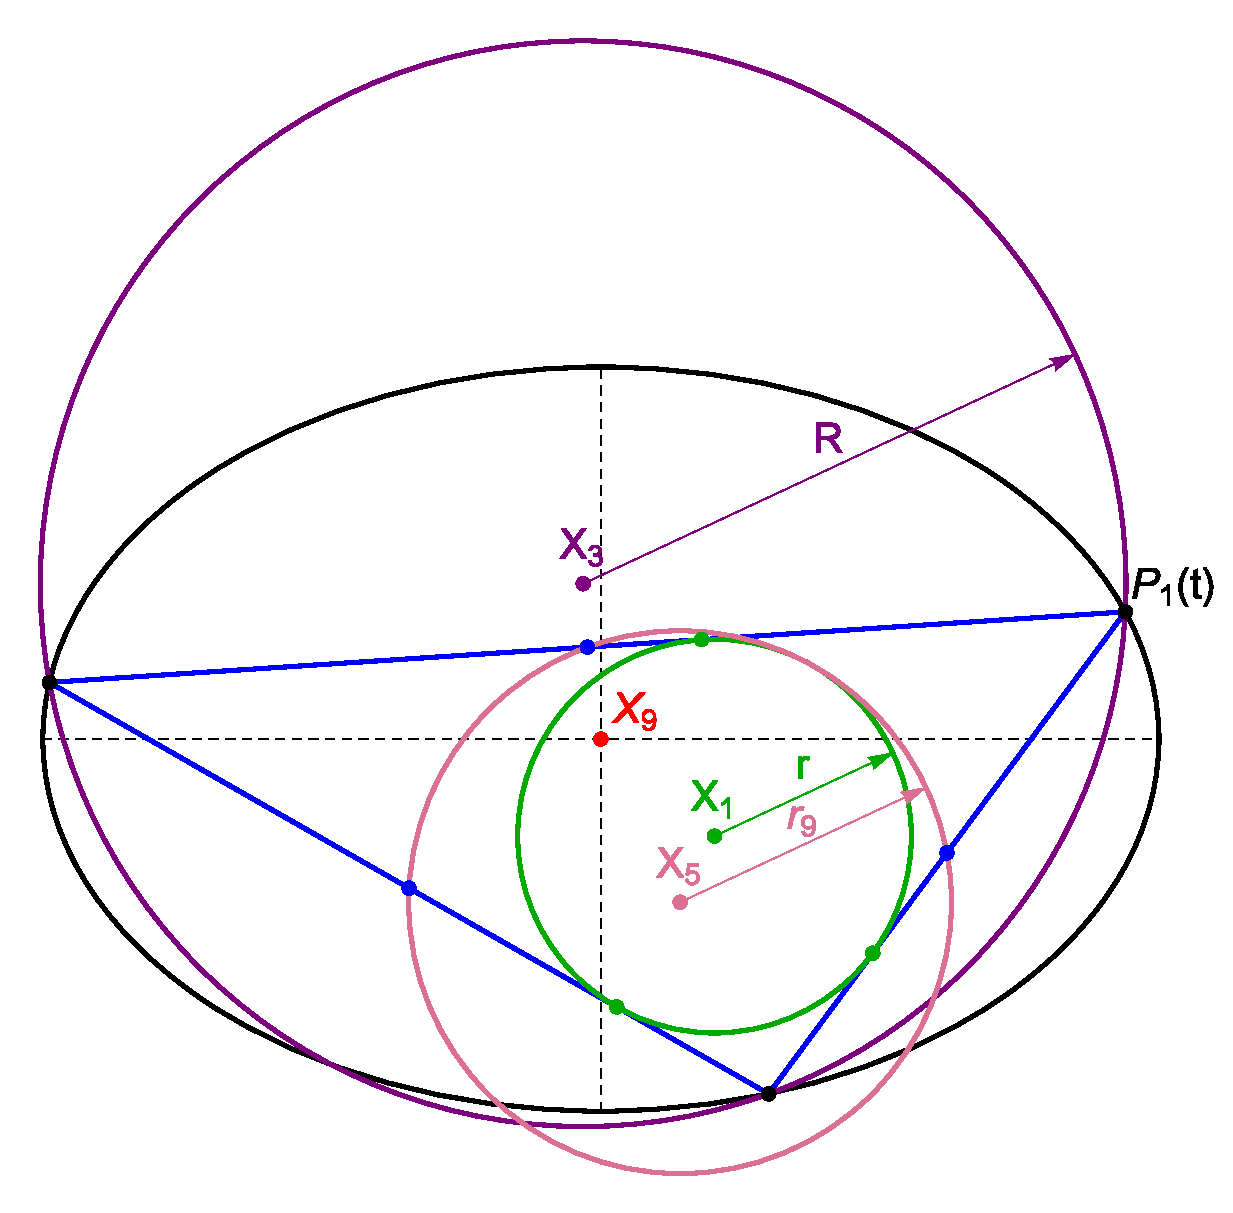
\includegraphics[width=\textwidth]{pics_03_100_radii}
    \caption{The incircle (green), circumcircle (purple), and 9-point (Euler's) circle (pink) of a billiard triangle (blue). These are centered on $X_1$, $X_3$, and $X_5$, respectively. Their radii are the inradius $r$, circumradius $R$, and 9-point circle radius $r_9=2R$. Over the family, the ratio $r/R=1+\sum\cos{\theta_i}$ is invariant.}
    \label{fig:radii}
\end{figure}

Let $\theta_i$, $r$, $R$, and $A$ denote the ith internal angle, inradius, circumradius, and area of a reference triangle. Primed quantities refer to the excentral triangle. The relations below hold for any triangle \cite{johnson29}. 

\begin{eqnarray}
\sum_{i=1}^{3}{\cos\theta_i}&=&1+\frac{r}{R} \label{eqn:sum-cos} \\
\prod_{i=1}^{3}{\cos\theta_i'}&=&\frac{r}{4R} \label{eqn:exc-prod-cos} \\
\frac{A}{A'}&=&\frac{r}{2R}
\label{eqn:area-ratio}
\end{eqnarray}

\begin{corollary}
Over billiard 3-periodics, also invariant are the sum of the orbit cosines, the product of excentral cosines, and the ratio of excentral-to-orbit areas.
\end{corollary}